\section{Results}
\label{sec:results}

Unless stated otherwise, all values in this section are from the selected model (version \RModelVersion, dataset build \RDatasetBuild, checkpoint \texttt{\RCheckpointShort\ldots}, seed \RSeed) and come from a single training run. Differences of a few percentage points between classes, sources or runs are within the range that seed-to-seed variation could produce and should not be read as established; the seed runs are reported in Section~\ref{sec:res-seeds}.

Run~2 was selected by the rule of Section~\ref{sec:selection}, because its macro-F1 on the common selection set was higher than that of run~1 (\RCmpRunTwoMacroFOne\% versus \RCmpRunOneMacroFOne\%); much of this advantage lies on sources that only run~2 trained on (Section~\ref{sec:res-runs}).

\subsection{Training}
Fig.~\ref{fig:curves} shows the training loss and the validation accuracy, macro-F1 and macro ROC-AUC per epoch. The run completed its full schedule of \REpochsTrained{} epochs (two head-only epochs followed by all configured phase-2 epochs); neither early stopping nor the wall-clock budget ended it. The checkpoint from epoch \RSelectedEpoch, the last epoch, had the highest validation macro-F1 and was selected, with validation accuracy \RValAcc\%, macro-F1 \RValMacroFOne\% and macro ROC-AUC \RValMacroAUC. The validation curve was still rising slightly at the end, so the run had not clearly plateaued; whether longer training would change the results was not tested.

\begin{figure}[t]
\centering
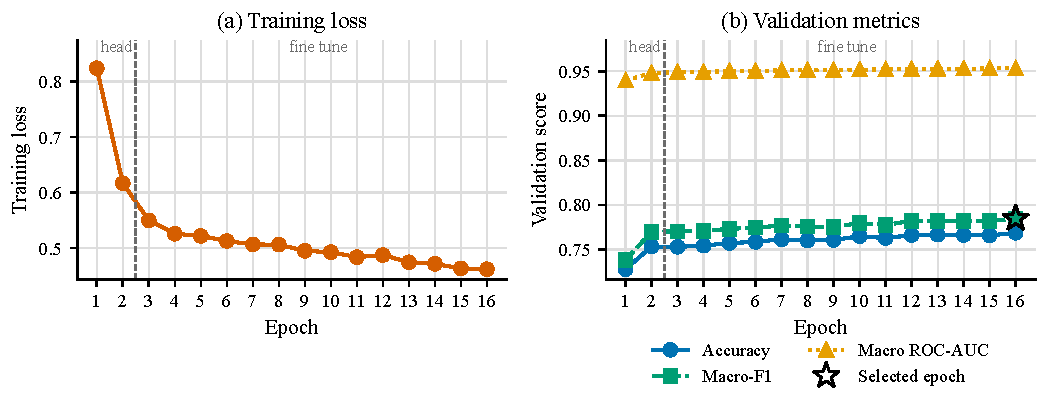
\includegraphics[width=\linewidth]{fig_training_curves.pdf}
\caption{Training loss and validation accuracy, macro-F1 and macro ROC-AUC per epoch for the selected run. Epochs 1--2: head only (backbone frozen); later epochs: last 30 backbone layers unfrozen.}
\label{fig:curves}
\end{figure}

\subsection{Overall internal performance}
Table~\ref{tab:overall} gives the validation and test results. On the internal test split ($N=\RNTest$), accuracy was \RTestAcc\% (Wilson 95\% CI \RTestAccLo--\RTestAccHi\%; percentile-bootstrap 95\% CI \RTestAccBootLo--\RTestAccBootHi\%), macro-F1 \RTestMacroFOne\%, weighted F1 \RTestWeightedFOne\%, macro precision \RTestMacroPrecision\%, macro recall \RTestMacroRecall\%, macro ROC-AUC \RTestMacroAUC{} and macro PR-AUC \RTestMacroPRAUC. Validation and test values are close (accuracy \RValAcc\% and \RTestAcc\%, macro ROC-AUC \RValMacroAUC{} and \RTestMacroAUC), so checkpoint selection on validation did not produce a visible optimistic bias for this split. The macro ROC-AUC is much higher than the threshold metrics: within the internal distribution the scores rank images of a class above images of other classes well, but the arg-max decision is wrong for about one test image in four, and most of these errors fall among a few classes (Section~\ref{sec:res-perclass}). A high ranking metric on internal data says nothing about whether the arg-max class is right on data from another hospital (Section~\ref{sec:res-ext}).

\begin{table}[t]
\centering
\caption{Overall results of the selected model. Validation was used for checkpoint selection; the test split was evaluated once. Accuracy CI: Wilson 95\%.}
\label{tab:overall}
\small
\begin{tabular}{@{}lrrrrr@{}}
\toprule
Split & $N$ & Accuracy (\%) & Macro-F1 (\%) & Macro ROC-AUC & Macro PR-AUC \\
\midrule
Validation & \RNVal & \RValAcc & \RValMacroFOne & \RValMacroAUC & -- \\
Test & \RNTest & \RTestAcc{} (\RTestAccLo--\RTestAccHi) & \RTestMacroFOne & \RTestMacroAUC & \RTestMacroPRAUC \\
\bottomrule
\end{tabular}
\end{table}

\subsection{Per-class performance}
\label{sec:res-perclass}
Table~\ref{tab:perclass} reports per-class metrics on the test split, Fig.~\ref{fig:cm} the confusion matrix, Fig.~\ref{fig:roc} the one-vs-rest ROC curves and Fig.~\ref{fig:perclass} precision, recall and F1 with recall confidence intervals.
The strongest classes by F1 were COVID-19 (\RFOneCovid\%), Tuberculosis (\RFOneTB\%) and Pneumonia (\RFOnePneumonia\%); COVID-19 and Tuberculosis also had the highest ROC-AUC (\RAUCCovid{} and \RAUCTB). The weakest were Pulmonary Nodule/Mass (F1 \RFOneNodule\%, ROC-AUC \RAUCNodule) and Normal (F1 \RFOneNormal\%). Most errors in the confusion matrix lie among Normal, Pleural Effusion and Nodule/Mass: Normal radiographs predicted as Nodule/Mass, and Nodule/Mass and Pleural Effusion confused with each other in both directions. Pleural Effusion and Nodule/Mass come only from NIH ChestX-ray14, whose labels were mined from radiology reports by natural language processing rather than read from the images; label noise and the subtlety of small nodules are both plausible contributors, which this study cannot separate. For the two small classes, high ROC-AUC did not come with low precision: COVID-19 and Tuberculosis had precision \RPrecisionCovid\% and \RPrecisionTB\%. The lowest precision was for Nodule/Mass (\RPrecisionNodule\%), the class into which most Normal errors fell.
% Confusion pattern: artifacts/evaluation_reports/model_metrics.json, internal_test.metrics.confusion_matrix (also fig_confusion_matrix).

\begin{table}[t]
\centering
\caption{Per-class results on the internal test split (one-vs-rest). Precision, recall, specificity and F1 in \%.}
\label{tab:perclass}
\small
\begin{tabular}{@{}lrrrrrr@{}}
\toprule
Class & Support & Precision & Recall & Specificity & F1 & ROC-AUC \\
\midrule
COVID-19              & \RSupportCovid     & \RPrecisionCovid     & \RRecallCovid     & \RSpecificityCovid     & \RFOneCovid     & \RAUCCovid \\
Normal                & \RSupportNormal    & \RPrecisionNormal    & \RRecallNormal    & \RSpecificityNormal    & \RFOneNormal    & \RAUCNormal \\
Pleural Effusion      & \RSupportEffusion  & \RPrecisionEffusion  & \RRecallEffusion  & \RSpecificityEffusion  & \RFOneEffusion  & \RAUCEffusion \\
Pneumonia             & \RSupportPneumonia & \RPrecisionPneumonia & \RRecallPneumonia & \RSpecificityPneumonia & \RFOnePneumonia & \RAUCPneumonia \\
Pulmonary Nodule/Mass & \RSupportNodule    & \RPrecisionNodule    & \RRecallNodule    & \RSpecificityNodule    & \RFOneNodule    & \RAUCNodule \\
Tuberculosis          & \RSupportTB        & \RPrecisionTB        & \RRecallTB        & \RSpecificityTB        & \RFOneTB        & \RAUCTB \\
\midrule
Macro average         & \RNTest            & \RTestMacroPrecision & \RTestMacroRecall & --                     & \RTestMacroFOne & \RTestMacroAUC \\
\bottomrule
\end{tabular}
\end{table}

\begin{figure}[t]
\centering
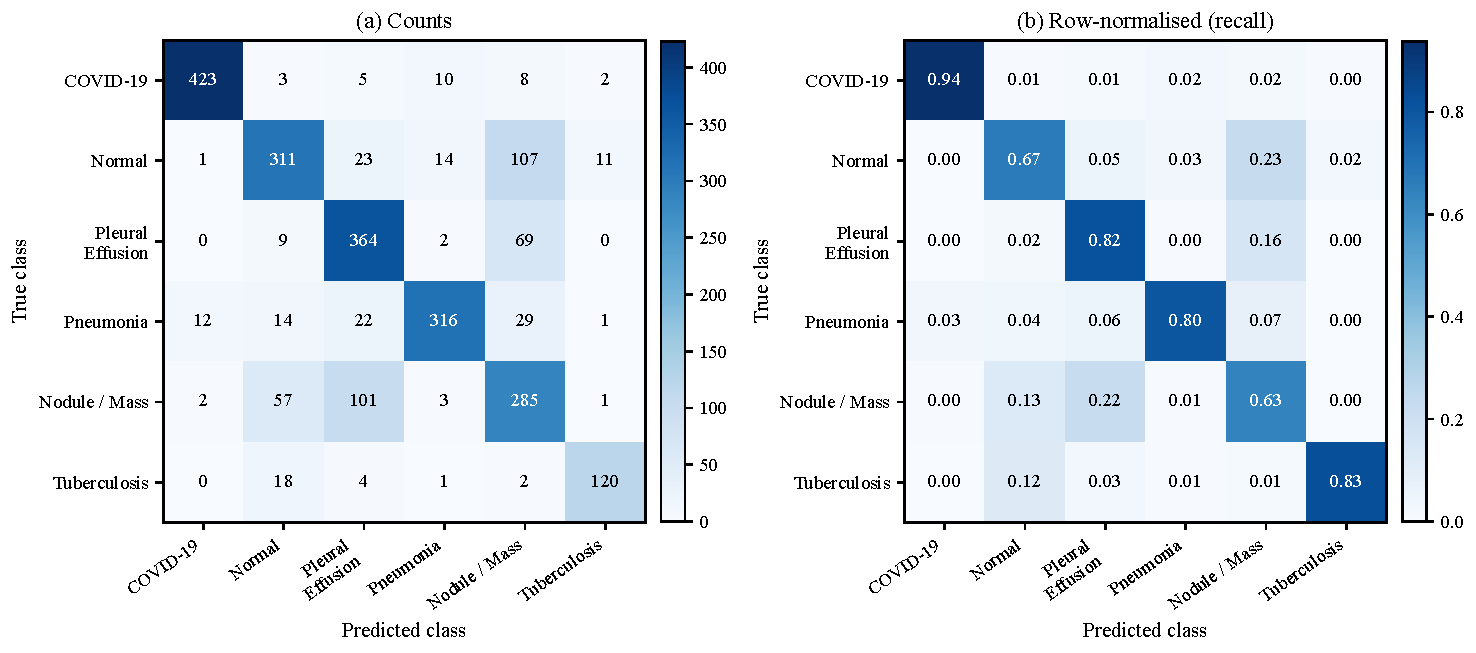
\includegraphics[width=\linewidth]{fig_confusion_matrix.pdf}
\caption{Confusion matrix on the internal test split: counts (left) and row-normalised (right). Rows: true class; columns: predicted class.}
\label{fig:cm}
\end{figure}

\begin{figure}[t]
\centering
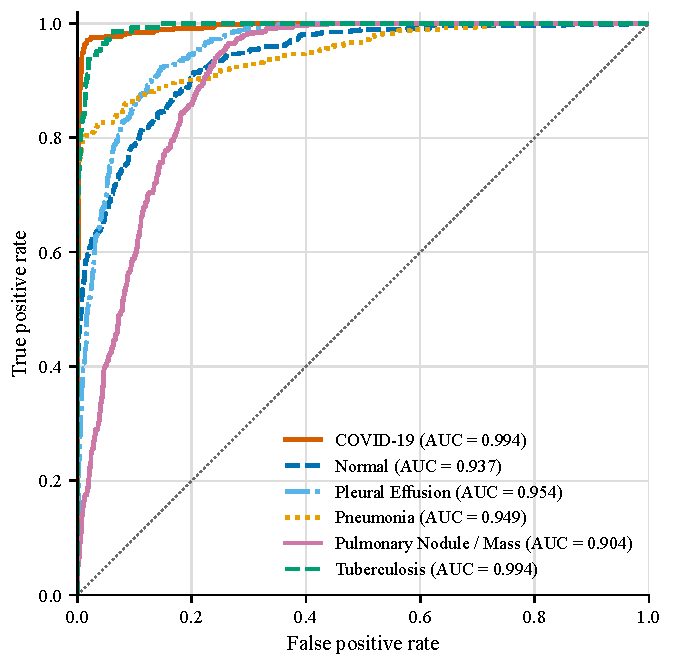
\includegraphics[width=0.8\linewidth]{fig_roc_curves.pdf}
\caption{One-vs-rest ROC curves per class on the internal test split, with per-class area under the curve.}
\label{fig:roc}
\end{figure}

\begin{figure}[t]
\centering
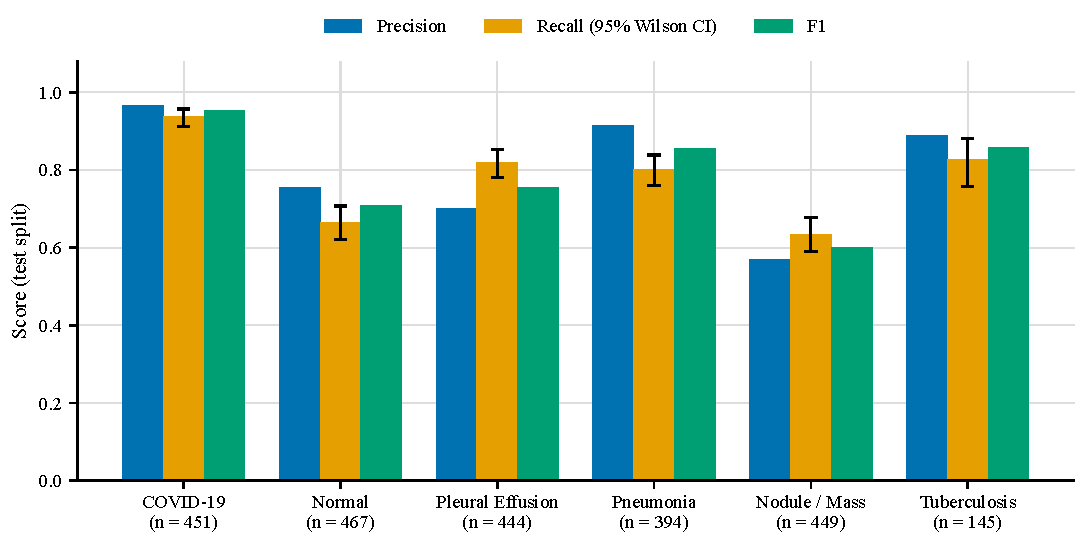
\includegraphics[width=\linewidth]{fig_per_class_metrics.pdf}
\caption{Precision, recall and F1 per class on the internal test split; error bars show Wilson 95\% confidence intervals for recall.}
\label{fig:perclass}
\end{figure}

\subsection{Performance by source}
\label{sec:res-source}
Table~\ref{tab:persource} and Fig.~\ref{fig:persource} give test accuracy within each source. Because several classes are supplied by one or two sources only, these values show how strongly the internal result depends on which collection an image came from; they are not measures of the quality of a source or of the diagnostic difficulty of its images.

\begin{table}[t]
\centering
\caption{Accuracy of the selected model within each source of the internal test split. ``Classes'' lists the classes that the source contributes to the test split.}
\label{tab:persource}
\small
\begin{tabular}{@{}llrr@{}}
\toprule
Source & Classes & $N$ & Accuracy (\%) \\
\midrule
NIH ChestX-ray14 & Normal, Effusion, Pneumonia, Nodule/Mass & \RSrcNNIH & \RSrcAccNIH \\
Kermany (paediatric) & Normal, Pneumonia & \RSrcNKermany & \RSrcAccKermany \\
COVID-19 Radiography Database & COVID-19 & \RSrcNCovidRad & \RSrcAccCovidRad \\
TBX11K & Normal, Tuberculosis & \RSrcNTBXk & \RSrcAccTBXk \\
Shenzhen & Normal, Tuberculosis & \RSrcNShenzhen & \RSrcAccShenzhen \\
COVID-19 image data collection & COVID-19, Normal, Pneumonia, TB & \RSrcNCohen & \RSrcAccCohen \\
\bottomrule
\end{tabular}
\end{table}

Accuracy ranged from \RSrcAccCohen\% (COVID-19 image data collection) to \RSrcAccCovidRad\% (COVID-19 Radiography Database), a source that contributes a single class. Kermany (paediatric Normal and Pneumonia) and TBX11K (Normal and Tuberculosis) reached \RSrcAccKermany\% and \RSrcAccTBXk\%, whereas NIH, which supplies four classes including the two NIH-only classes, reached \RSrcAccNIH\%. The overall test accuracy of \RTestAcc\% is a weighted mixture of these values and would change with the source mix. The same class was also recognised very differently depending on its source: Normal radiographs from NIH were called Normal far less often than Normal radiographs from Kermany, Shenzhen or TBX11K. This pattern is consistent with source-specific appearance contributing to the decisions, but per-source accuracy alone cannot separate a source effect from differences in case mix; Section~\ref{sec:res-probe} addresses this more directly.
% Within-source class recall: artifacts/evaluation_reports/model_metrics.json, internal_test.per_source.<source>.recall_by_class (not in the macro file).

\begin{figure}[t]
\centering
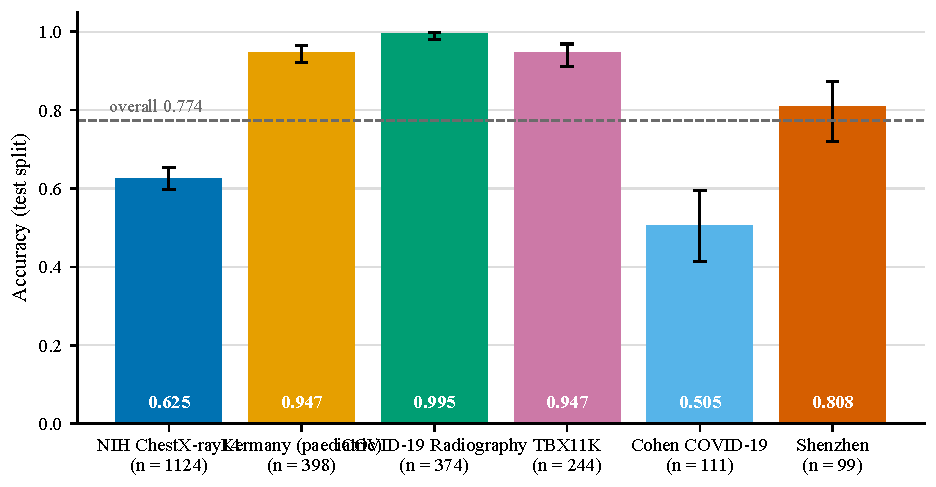
\includegraphics[width=0.85\linewidth]{fig_per_source.pdf}
\caption{Accuracy on the internal test split within each source. A source that is the only provider of a class can be recognised by its image style rather than by disease, so these values are not comparable with one another as measures of diagnostic difficulty.}
\label{fig:persource}
\end{figure}

\subsection{Source-identifiability probe}
\label{sec:res-probe}
Table~\ref{tab:probe} gives the balanced accuracy with which the linear probe of Section~\ref{sec:probe} predicted the source of the \RProbeNTest{} probe-test images. With ImageNet features, which contain nothing learned from this project, the source was identified with balanced accuracy \RProbeImgBalAcc\% across \RProbeImgNSources{} sources (chance \RProbeImgChance\%). The source remained identifiable within single classes: among Normal images \RProbeImgWithinNormal\% across \RProbeImgWithinNormalNSources{} sources (chance \RProbeImgWithinNormalChance\%), among Tuberculosis images \RProbeImgWithinTB\% (chance \RProbeImgWithinTBChance\%), among Pneumonia images \RProbeImgWithinPneumonia\% (chance \RProbeImgWithinPneumoniaChance\%) and among COVID-19 images \RProbeImgWithinCovid\% (chance \RProbeImgWithinCovidChance\%). Features from the trained model's backbone gave nearly identical values (\RProbeMdlBalAcc\% overall). This is expected: fine-tuning changed only the last 17 weighted layers of the backbone, so its features remain close to the ImageNet features (verified by comparing the weights).

\begin{table}[t]
\centering
\caption{Source-identifiability probe: balanced accuracy (\%) of a logistic regression predicting the source collection from frozen 1024-dimensional features, on \RProbeNTest{} probe-test images (\RProbeNTrain{} probe-training images). ``Within'' rows use only images of that class. Chance is $1/S$ for $S$ sources.}
\label{tab:probe}
\small
\begin{tabular}{@{}lrrrr@{}}
\toprule
Images & Sources & Chance & ImageNet features & Trained backbone \\
\midrule
All classes & \RProbeImgNSources & \RProbeImgChance & \RProbeImgBalAcc & \RProbeMdlBalAcc \\
Within Normal & \RProbeImgWithinNormalNSources & \RProbeImgWithinNormalChance & \RProbeImgWithinNormal & \RProbeMdlWithinNormal \\
Within Tuberculosis & \RProbeImgWithinTBNSources & \RProbeImgWithinTBChance & \RProbeImgWithinTB & \RProbeMdlWithinTB \\
Within Pneumonia & \RProbeImgWithinPneumoniaNSources & \RProbeImgWithinPneumoniaChance & \RProbeImgWithinPneumonia & \RProbeMdlWithinPneumonia \\
Within COVID-19 & \RProbeImgWithinCovidNSources & \RProbeImgWithinCovidChance & \RProbeImgWithinCovid & \RProbeMdlWithinCovid \\
\bottomrule
\end{tabular}
\end{table}

Because each source supplies a different subset of classes (Table~\ref{tab:persource}), source and class are confounded in this benchmark, and the probe shows that source information is linearly available in the very features on which the classifier's head operates. A source shortcut is therefore possible. The probe does not show that the classifier uses it; that conclusion would need an intervention such as leave-one-source-out training, which was not performed. We treat the probe as indirect evidence and interpret it only together with the per-source results above, the external breakdown (Section~\ref{sec:res-ext}) and the Grad-CAM examples (Section~\ref{sec:res-gradcam}).

\subsection{Calibration}
The expected calibration error on the test split was \RTestECE{} (15 equal-width bins; Eq.~\eqref{eq:ece}); Fig.~\ref{fig:calib} shows the reliability diagram. The highest-score bin holds the largest share of test images and lies close to the diagonal. In several bins of the middle score range accuracy is somewhat below the mean score, a mild over-confidence, and incorrect predictions have a clearly lower mean top-class score than correct ones. A low ECE on the internal test split does not imply calibrated scores on data from another hospital, where, as shown below, the arg-max class is often wrong. No calibration map was fitted, and the 0.5 ``inconclusive'' threshold used by the application has not been validated.
% Source: artifacts/evaluation_reports/model_metrics.json, internal_test.metrics.calibration (bins, mean_confidence_correct, mean_confidence_incorrect).

\begin{figure}[t]
\centering
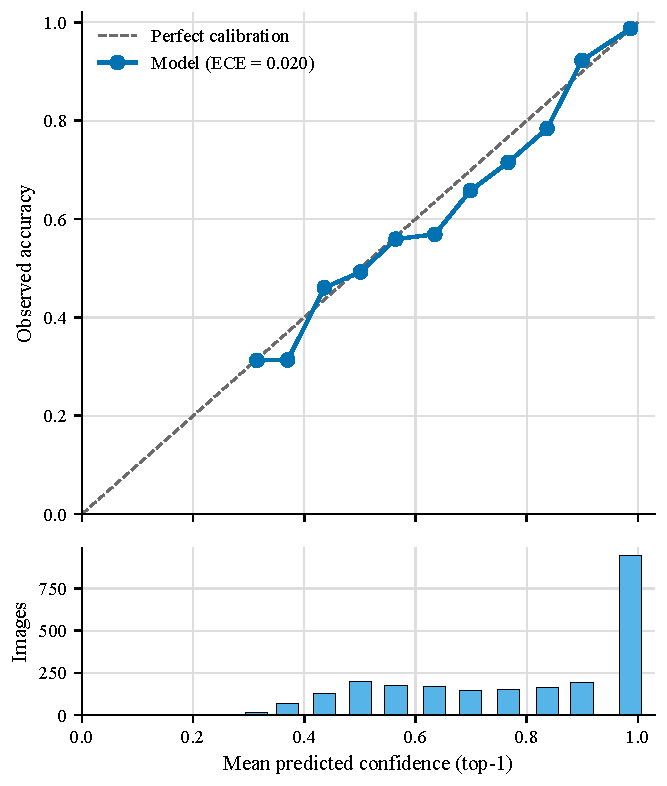
\includegraphics[width=0.6\linewidth]{fig_calibration.pdf}
\caption{Reliability diagram on the internal test split: accuracy versus mean top-class softmax score in 15 equal-width bins. The diagonal is perfect calibration.}
\label{fig:calib}
\end{figure}

\subsection{External cohort}
\label{sec:res-ext}
Table~\ref{tab:external} and Fig.~\ref{fig:external} give the results on the Montgomery cohort ($N=\RNExternal$). Of the \RExtSensN{} TB radiographs, \RExtSensK{} were predicted as some class other than Normal (sensitivity \RExtSens\%, 95\% CI \RExtSensLo--\RExtSensHi\%); of the \RExtSpecN{} normal radiographs, \RExtSpecK{} were predicted Normal (specificity \RExtSpec\%, 95\% CI \RExtSpecLo--\RExtSpecHi\%). The ROC-AUC of the abnormality score $1-p_{\text{Normal}}$ was \RExtAUC. Exactly \RExtTBK{} of \RExtTBN{} TB radiographs (\RExtTB\%) were assigned the Tuberculosis class. The model assigned COVID-19 to \RExtCovidCalls{} of the \RNExternal{} external radiographs, although the cohort contains no COVID-19 cases.

Fig.~\ref{fig:external} shows where the errors went. Most Montgomery radiographs, normal and TB alike, were assigned Pneumonia or Pulmonary Nodule/Mass, and some TB radiographs Pleural Effusion. The high sensitivity is therefore not TB detection: the TB scans were called abnormal, but with a disease the cohort does not contain, while the internal Tuberculosis recall was \RRecallTB\%. The low specificity means that the model would flag most healthy patients from this hospital as abnormal. That the ROC-AUC of $1-p_{\text{Normal}}$ (\RExtAUC) is well above chance while specificity is low indicates that the scores still order TB scans above normal scans to some degree, but the decision boundary learned on the development sources does not transfer.

Run~1, which had seen COVID-19 only from the COVID-19 image data collection, behaved differently on the same cohort, also evaluated once: it assigned COVID-19 to \RRunOneExtCovidCalls{} of the \RNExternal{} Montgomery radiographs, called \RRunOneExtSpecK{} of the \RExtSpecN{} normal radiographs Normal and named \RRunOneExtTBK{} of the \RExtTBN{} TB radiographs Tuberculosis.
With build~2, which added TBX11K, the COVID-19 Radiography Database and two further NIH archives at once, the COVID-19 calls on Montgomery fell from \RRunOneExtCovidCalls{} to \RExtCovidCalls. This is consistent with, but does not prove, run~1 having associated the appearance of its single COVID-19 source with the class; build~2 changed several sources together, so the change cannot be attributed to one of them. The external errors did not become correct, however: they moved to other abnormal classes, specificity was lower than run~1's, and Tuberculosis was still not recognised, although Tuberculosis in build~2 also comes from two sources. The internal gains of run~2 did not translate into better external specificity or any TB recognition. These are single-seed observations on one small cohort.

\begin{table}[t]
\centering
\caption{External cohort (Montgomery County; binary normal vs TB; evaluated once). ``Abnormal'' means any predicted class other than Normal. CIs: Wilson 95\%.}
\label{tab:external}
\small
\begin{tabular}{@{}lrr@{}}
\toprule
Quantity & Count & \% (95\% CI) \\
\midrule
TB scans predicted abnormal (sensitivity) & \RExtSensK/\RExtSensN & \RExtSens{} (\RExtSensLo--\RExtSensHi) \\
Normal scans predicted Normal (specificity) & \RExtSpecK/\RExtSpecN & \RExtSpec{} (\RExtSpecLo--\RExtSpecHi) \\
TB scans predicted Tuberculosis (exact TB recall) & \RExtTBK/\RExtTBN & \RExtTB \\
All scans predicted COVID-19 & \RExtCovidCalls/\RNExternal & -- \\
ROC-AUC of $1-p_{\text{Normal}}$ & \multicolumn{2}{r}{\RExtAUC} \\
\bottomrule
\end{tabular}
\end{table}

\begin{figure}[t]
\centering
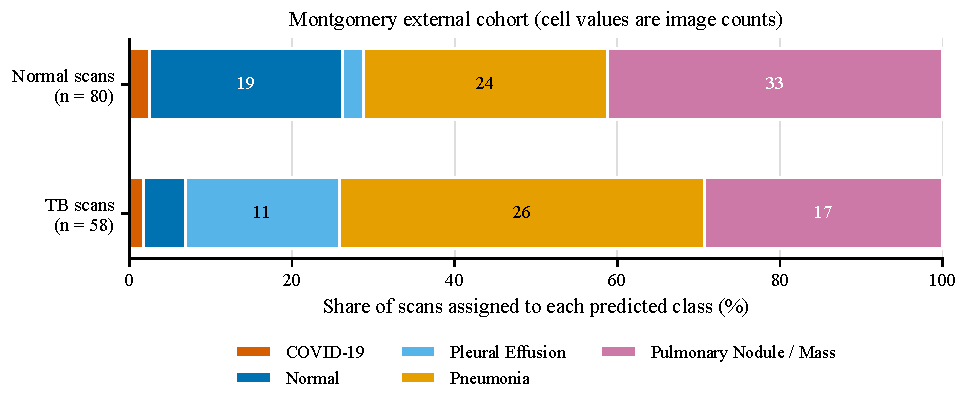
\includegraphics[width=\linewidth]{fig_external_breakdown.pdf}
\caption{Predicted class for the normal (left) and TB (right) radiographs of the external Montgomery cohort. The cohort contains no COVID-19, Pleural Effusion, Pneumonia or Nodule/Mass cases.}
\label{fig:external}
\end{figure}

\subsection{Comparison of run 1 and run 2}
\label{sec:res-runs}
Table~\ref{tab:runs} compares the two runs on the common selection set defined in Section~\ref{sec:selection} and reports each run's once-only test and external results for completeness. Test rows are not comparable between runs, because the two builds have different test splits, and neither test nor external rows were used for selection.

\begin{table}[t]
\centering
\caption{Comparison of run~1 (build~1) and run~2 (build~2). Selection used only the macro-F1 on the common selection set. Shared sources: NIH, Kermany, Shenzhen and the COVID-19 image data collection, on which both runs trained. Single seed per run; the McNemar test is descriptive. Percentages except ROC-AUC.}
\label{tab:runs}
\small
\begin{tabular}{@{}lll@{}}
\toprule
Quantity & Run 1 & Run 2 \\
\midrule
Common set: $N$ & \multicolumn{2}{c}{\RCmpN} \\
Common set: macro-F1 (selection criterion) & \RCmpRunOneMacroFOne & \RCmpRunTwoMacroFOne \\
Common set: macro ROC-AUC & \RCmpRunOneMacroAUC & \RCmpRunTwoMacroAUC \\
Common set: accuracy & \RCmpRunOneAcc & \RCmpRunTwoAcc \\
Shared sources only: $N$ & \multicolumn{2}{c}{\RCmpRunOneSharedN} \\
Shared sources only: macro-F1 & \RCmpRunOneSharedMacroFOne & \RCmpRunTwoSharedMacroFOne \\
Shared sources only: macro ROC-AUC & \RCmpRunOneSharedMacroAUC & \RCmpRunTwoSharedMacroAUC \\
Shared sources only: accuracy & \RCmpRunOneSharedAcc & \RCmpRunTwoSharedAcc \\
Exact McNemar test, all common images & \multicolumn{2}{c}{\RCmpMcNemarB{} vs \RCmpMcNemarC{} discordant; $p=\RCmpMcNemarP$} \\
\midrule
Own test split: $N$ & \RRunOneTestN & \RNTest \\
Own test split: accuracy / macro-F1 & \RRunOneTestAcc{} / \RRunOneTestMacroFOne & \RTestAcc{} / \RTestMacroFOne \\
Own test split: macro ROC-AUC & \RRunOneTestMacroAUC & \RTestMacroAUC \\
External: sensitivity / specificity & \RRunOneExtSensK/\RExtSensN{} / \RRunOneExtSpecK/\RExtSpecN & \RExtSensK/\RExtSensN{} / \RExtSpecK/\RExtSpecN \\
External: ROC-AUC of $1-p_{\text{Normal}}$ & \RRunOneExtAUC & \RExtAUC \\
External: exact TB recall; COVID-19 calls & \RRunOneExtTBK/\RExtTBN; \RRunOneExtCovidCalls & \RExtTBK/\RExtTBN; \RExtCovidCalls \\
\midrule
Selected & & \checkmark{} (\RCmpSelected) \\
\bottomrule
\end{tabular}
\end{table}
% McNemar: first count = run 1 right and run 2 wrong; second = run 1 wrong and run 2 right.

By the rule of Section~\ref{sec:selection}, which was fixed in advance and recorded in the repository before run~2's results existed (run~2 itself was started after run~1's external results had been seen), run~2 was selected: its macro-F1 on the \RCmpN{} common images was \RCmpRunTwoMacroFOne\% against \RCmpRunOneMacroFOne\% for run~1, with accuracy \RCmpRunTwoAcc\% against \RCmpRunOneAcc\% and macro ROC-AUC \RCmpRunTwoMacroAUC{} against \RCmpRunOneMacroAUC. Of the paired predictions that differed in correctness, \RCmpMcNemarB{} were right for run~1 only and \RCmpMcNemarC{} for run~2 only (exact McNemar $p=\RCmpMcNemarP$), a statistic we report as descriptive.

\textbf{This comparison favours run~2 by construction, and the size of the gap should not be read as the effect of a better training recipe.} The common set includes TBX11K and COVID-19 Radiography images, which are in-distribution for run~2 and unseen for run~1. Restricted to the \RCmpRunOneSharedN{} common images from the four sources both runs trained on, the two runs had almost the same accuracy (\RCmpRunOneSharedAcc\% and \RCmpRunTwoSharedAcc\%) and the same macro ROC-AUC (\RCmpRunOneSharedMacroAUC{} and \RCmpRunTwoSharedMacroAUC), and the macro-F1 gap was much smaller (\RCmpRunOneSharedMacroFOne\% and \RCmpRunTwoSharedMacroFOne\%). Much of run~2's advantage therefore lies on the sources that only run~2 trained on. The selection rule was fixed before run~2's results were known, but run~2 itself was started after run~1's external results had been seen (Section~\ref{sec:design}). On the external cohort, the one data set that neither run trained on, run~2 removed run~1's COVID-19 calls but did not improve specificity (Section~\ref{sec:res-ext}). With one seed per run, none of these differences is evidence that one recipe is better in general.

\subsection{Seed variability}
\label{sec:res-seeds}
Table~\ref{tab:seeds} reports the selected run and the two follow-up seeds of Section~\ref{sec:followup}, each evaluated once on the test split and the external cohort. \pending{seed variability: size of the seed-to-seed spread of test accuracy, macro-F1, macro ROC-AUC, external specificity and exact TB recall; whether the selected run lies inside the spread; which earlier statements (class, source and run differences) are smaller than the spread. Use \texttt{\textbackslash RMS...} macros only}.

\begin{table}[t]
\centering
\caption{Seed variability of the selected configuration (build \RDatasetBuild). Test values in \%, except ROC-AUC; external specificity and exact Tuberculosis recall in \%. Mean $\pm$ sample SD over the three runs. The served model is run~2 regardless of these results.}
\label{tab:seeds}
\small
\begin{tabular}{@{}llrrrrr@{}}
\toprule
Run & Seed & Test acc. & Macro-F1 & Macro ROC-AUC & Ext. specificity & Ext. TB recall \\
\midrule
Run 2 (selected) & \RSeed & \RTestAcc & \RTestMacroFOne & \RTestMacroAUC & \RExtSpec & \RExtTB \\
% Run 2 row = \RMSRunOne... (Seed, TestAcc, TestMacroFOne, TestMacroAUC, ExtSens, ExtSpec, ExtTB); values identical to the macros used here.
Run 3 & 43 % \RMSRunTwoSeed
  & \pending{} % \RMSRunTwoTestAcc
  & \pending{} % \RMSRunTwoTestMacroFOne
  & \pending{} % \RMSRunTwoTestMacroAUC
  & \pending{} % \RMSRunTwoExtSpec
  & \pending{} % \RMSRunTwoExtTB
  \\
Run 4 & 44 % \RMSRunThreeSeed
  & \pending{} % \RMSRunThreeTestAcc
  & \pending{} % \RMSRunThreeTestMacroFOne
  & \pending{} % \RMSRunThreeTestMacroAUC
  & \pending{} % \RMSRunThreeExtSpec
  & \pending{} % \RMSRunThreeExtTB
  \\
\midrule
Mean $\pm$ SD & --
  & \pending{} % \RMSTestAccMean $\pm$ \RMSTestAccSD
  & \pending{} % \RMSTestMacroFOneMean $\pm$ \RMSTestMacroFOneSD
  & \pending{} % \RMSTestMacroAUCMean $\pm$ \RMSTestMacroAUCSD
  & \pending{} % \RMSExtSpecMean $\pm$ \RMSExtSpecSD
  & \pending{} % \RMSExtTBMean $\pm$ \RMSExtTBSD
  \\
\bottomrule
\end{tabular}
\end{table}
% Fill the Mean +/- SD row with \RMSTestAccMean $\pm$ \RMSTestAccSD, \RMSTestMacroFOneMean $\pm$ \RMSTestMacroFOneSD,
% \RMSTestMacroAUCMean $\pm$ \RMSTestMacroAUCSD, \RMSExtSpecMean $\pm$ \RMSExtSpecSD, \RMSExtTBMean $\pm$ \RMSExtTBSD
% (also available: \RMS<metric>Min/Max, \RMSExtSensMean/SD, \RMSExtAUCMean/SD, \RMSNRuns, \RMSSeeds).
% Per-run macros (after aggregation): \RMSRun<One|Two|Three><Seed|TestAcc|TestMacroFOne|TestMacroAUC|ExtSens|ExtSpec|ExtTB>, One = run 2, Two = run 3, Three = run 4.

\subsection{Preprocessing ablation}
\label{sec:res-ablation}
Table~\ref{tab:ablation} compares the selected run, trained with the full filtering chain, with run~5, trained with the same seed, data and schedule but without the Gaussian pre-blur, CLAHE and low-pass filter. \pending{ablation: direction and size of the differences on test and external data, read against the seed spread of Table~\ref{tab:seeds}; no claim that the filtering helps or harms unless the difference clearly exceeds that spread. Use \texttt{\textbackslash RAbl...} macros only}.

\begin{table}[t]
\centering
\caption{Preprocessing ablation: full chain (run~2) versus no filtering (run~5), same seed (\RSeed), build, split and schedule. One run each; compare differences with the seed spread in Table~\ref{tab:seeds}. Percentages except ROC-AUC.}
\label{tab:ablation}
\small
\begin{tabular}{@{}lrr@{}}
\toprule
Quantity & Run 2 (full chain) & Run 5 (no filters) \\
\midrule
Test accuracy & \RTestAcc & \pending{} \\
Test macro-F1 & \RTestMacroFOne & \pending{} \\
Test macro ROC-AUC & \RTestMacroAUC & \pending{} \\
External sensitivity & \RExtSens & \pending{} \\
External specificity & \RExtSpec & \pending{} \\
External exact TB recall & \RExtTB & \pending{} \\
\bottomrule
\end{tabular}
\end{table}
% Fill run-5 cells with \RAblTestAcc, \RAblTestMacroFOne, \RAblTestMacroAUC, \RAblExtSens, \RAblExtSpec, \RAblExtTB.

\subsection{Grad-CAM examples}
\label{sec:res-gradcam}
Fig.~\ref{fig:gradcam} shows Grad-CAM maps for one test image per class, chosen by the rule fixed before any heatmap was viewed (Section~\ref{sec:methods}): the correctly classified image with the median top-class score of its class. In these examples the COVID-19 and Normal heatmaps concentrate on the neck and trachea, the shoulders and the image borders rather than the lung fields; the Nodule/Mass and Tuberculosis heatmaps fall inside the lung fields; and the Pneumonia example, a paediatric image from the Kermany collection, is diffuse. With one image per class these maps are illustrative only. Attention outside the lungs for COVID-19 and Normal is consistent with acquisition or source cues contributing to those decisions, but it does not establish it, and saliency maps on chest radiographs are themselves unreliable~\cite{arun2021assessing}.

\begin{figure}[t]
\centering
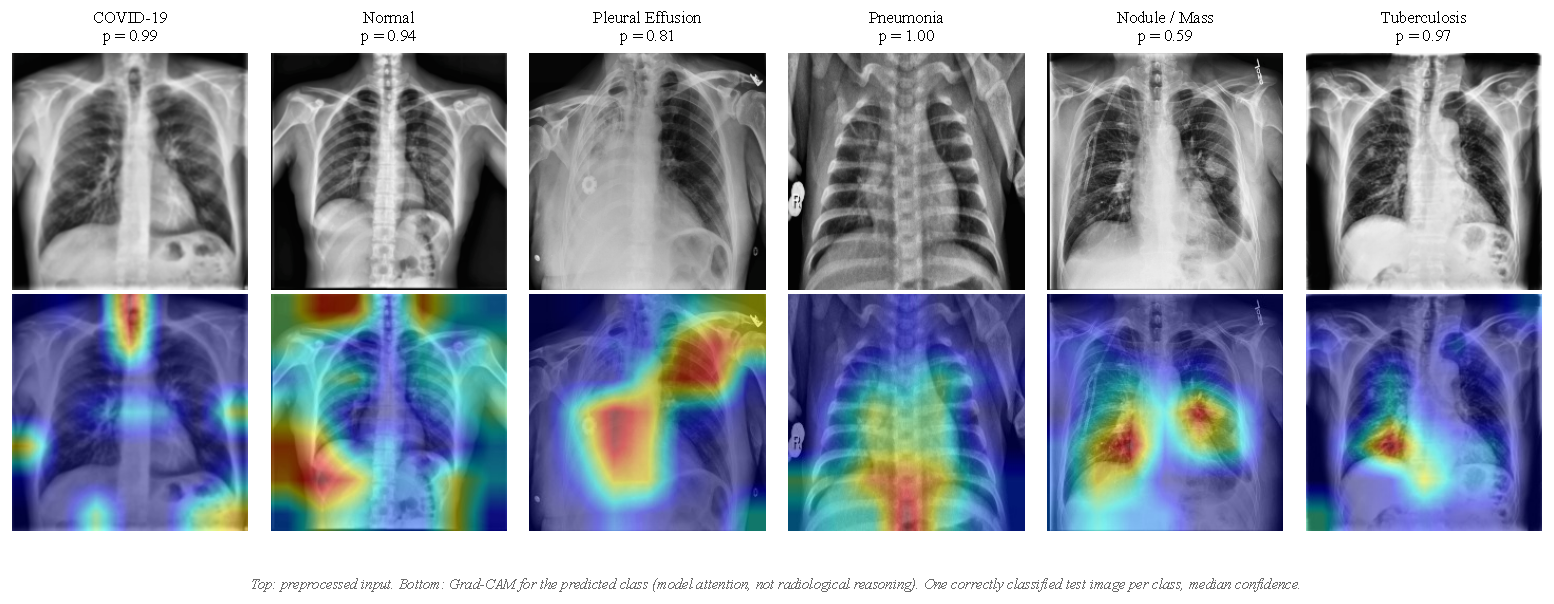
\includegraphics[width=\linewidth]{fig_gradcam_examples.pdf}
\caption{Grad-CAM maps for the predicted class on one correctly classified test radiograph per class, each the image with the median top-class score among the correct predictions of its class (rule fixed before viewing). The maps show which regions influenced the class score; they do not show radiological reasoning.}
\label{fig:gradcam}
\end{figure}
